% https://www.reddit.com/r/EngineeringResumes/wiki/index

\documentclass{friggeri}
\usepackage{multicol}
\usepackage{changepage}
\usepackage{etoolbox}
\usepackage{enumitem}
\usepackage{siunitx}
\sisetup{detect-all,group-separator = {,}, per-mode=repeated-symbol}

% Match double quotes
% https://tex.stackexchange.com/a/52354
\usepackage [english]{babel}
\usepackage [autostyle, english = american]{csquotes}
\MakeOuterQuote{"}

\usepackage{hyperref}
\hypersetup{
	allbordercolors=blue,
	pdfborderstyle={/S/U/W 1},
}

% Toggle personal contact information for web version
\newbool{forweb}
\setbool{forweb}{false}

\setlength{\columnsep}{0cm}


% header and footer
\pagestyle{fancy}
% Clear the header and footer
\fancyhf{}
% remove top line
\renewcommand{\headrulewidth}{0pt}
% Set the right side of the footer to be the page number
\fancyfoot[C]{\footnotesize \thepage\ of \pageref*{LastPage}}
% \rhead{{\tiny \addfontfeature{Color=lightgray}Current as of \\ \today}}
\rhead{\footnotesize \addfontfeature{Color=lightgray} Current as of \\ \today}


\begin{document}

% \header{chris}{leaman}{chartered maritime \& coastal engineer}
% \vspace{-1.0cm} % ADJUST THIS TO PUSH CONTENTS UP/DOWN THE PAGE

\section{{\LARGE Dr. Chris Leaman} \small{ PhD, BEng, CPEng, RPEQ, NER}}

\entryitemindent{
\begin{tabularx}{\linewidth}{X l p{7cm}}
   Brisbane, QLD, Australia  & \href{mailto:ckleaman@gmail.com}{ckleaman@gmail.com} & \\ 
   Australian Citizen (NV1 Security Clearance)  & +61 488 404 949 & \\
   British Citizen & & 
\end{tabularx}
}

% \section{professional summary}
\begin{adjustwidth}{2cm}{}
  Current PhD Student at UNSW WRL, investigating regional scale storm wave forecasting in the context of an Australian coastal hazards Early Warning System.
  Chartered Professional coastal and maritime engineer (CPEng \& RPEQ) with a variety of extensive skills in structural engineering, coastal modelling, and hydraulic modelling.
  Seven years of diverse experience as an engineering consultant, demonstrating adaptability and flexibility to work effectively in autonomous and team environments.\\
  \vspace{-2\parskip}
\end{adjustwidth}


\section{positions held}

\begin{entrylist}

\entry%
{2017--18\\
2011--16}
{\vspace*{-4.6ex}\\Structural Engineer (Maritime \& Coastal)\\
Graduate Structural Engineer (Maritime \& Coastal)}%
{Brisbane, Queensland}
{\emph{Kellogg, Brown \& Root}}

& Key skills and responsibilities:\\

\entrybulletsindented%
{}
{Coastal, hydraulic and hydrologic modelling}
{}
{\begin{itemize}
\item Modelling coastal processes including waves and sediment transport using DELFT3D
\item Building and developing TUFLOW models to simulate flood events
\item Developing flood studies and risk assessments for regional towns and rail tracks
\end{itemize}
}

\entrybulletsindented%
{}
{Structural engineering of maritime structures}
{}
{\begin{itemize}
  \item Completing structural design and detailing of wharves, dolphins, sea walls and ramps
  \item Performing complex finite element analysis using Strand7
  \item Inspecting site works for design verification and construction support purposes
\end{itemize}
}

\entrybulletsindented%
{}
{Programming and documentation}
{}
{\begin{itemize}
\item Developing Excel VBA and Python scripts to perform large scale, complex analysis
\item Writing technical reports, specification and proposal documents

\end{itemize}}



%------------------------------------------------
\end{entrylist}

\section{Skills}

\entryitemindent{
	\textbf{Structural engineering design:} Reinforced concrete, steel, timber, piles, retaining walls, footings \\
   \textbf{Maritime structural engineering:} Wharves, jetties, dolphins, seawalls, berthing, mooring, wave loading, seismic loading \\ 
   \textbf{Coastal process and coastal management:} Hydrodynamic modelling, overtopping, coastal erosion, breakwaters, revetments\\
   % \textbf{Construction:} Supervision, site support, contractor management \\
   \textbf{Software and programming:} SPACEGASS, Strand7, Optimoor, Machine Learning, Python, QGIS, \LaTeX\\
   \textbf{Management:} Project management, design management, team management\\ 
   % \textbf{Business development:} \\ 
}

\section{Education}

	\entrytable%
	{Doctor of Philosophy}
	{2022}
	{}
	{The University of New South Wales --- Water Research Laboratory}
	{Sydney, New South Wales}
	{\begin{itemize}
			\item Supported by the UNSW Scientia PhD Scholarship Scheme.
			\item Thesis title: \href{https://unsworks.unsw.edu.au/entities/publication/dd04df5e-b0bf-4114-b408-4961af02c852}{\textit{``Regional-Scale Forecasting for Coastal Storm Impact Early Warning Systems''.}}
			\item Recipient of the \href{https://www.inside.unsw.edu.au/awards/2022-deans-awards-outstanding-phd-theses}{``Dean's Award for Outstanding PhD Thesis''}.
		\end{itemize}
	}

	\entrytable%
	{Bachelor of Engineering {\normalfont (Extended Major in Civil Engineering)}}
	{2010}
	{}
	{The University of Queensland}
	{Brisbane, Queensland}
	{\vspace{-3\parskip}}

\section{professional memberships}
\begin{entrylist}
%------------------------------------------------
\entry%
{since 2017}
{Chartered Professional Engineer {\normalfont (CPEng) (Structural)}\\
National Engineering Register {\normalfont (NER) (Structural)}}%
{}
{\emph{Engineers Australia}
}
%------------------------------------------------
\end{entrylist}

\newpage
\section{Career Project Highlights}
\small{\textit{The following projects have significantly contributed to my experience as a maritime and coastal engineer:}}
\renewcommand{\topfraction}{.999}
\renewcommand{\floatpagefraction}{.999}%
\fboxsep=0pt%padding thickness
\fboxrule=0.5pt%border thickness

\FloatBarrier
\begin{table}[h!]
    \begin{tblr}{Q[halign=l,valign=h,wd=0.63\textwidth]Q[halign=r,valign=t]}
    {\entrytableprojecthighlight%
	{ESTDEF01PH01 AUKUS Submarine Rotational Force -- West}
	{2023 to Present}
	{}
	{Maritime Structures Lead for KBR}
	{Perth, Western Australia}
	{Client: Australian Department of Defence}
	{\vspace{1em}\begin{itemize}
		 \item From as early as 2027, AUKUS partners will have a rotational presence at HMAS \textit{Stirling} of UK and US nuclear-powered submarines -- known as 'Submarine Rotational Force-West'
		 \item Technical oversight of maritime structure infrastructure upgrades, including potential wharf strengthening work, new fender frames, dredging and associated small craft facilities. 
		 \item Exposure to nuclear safety related design process, including risk assessments, hazard identification and nuclear safety justification documentation.
		 \item Significant amounts of multi-disciplinary coordination due to the large amount of services required to maintain the vessels.
		 \item Managed design to tight delivery schedule, given the commitments from the government and significant public interest in the project.
	 \end{itemize}}
	} & \fcolorbox{black}{black}{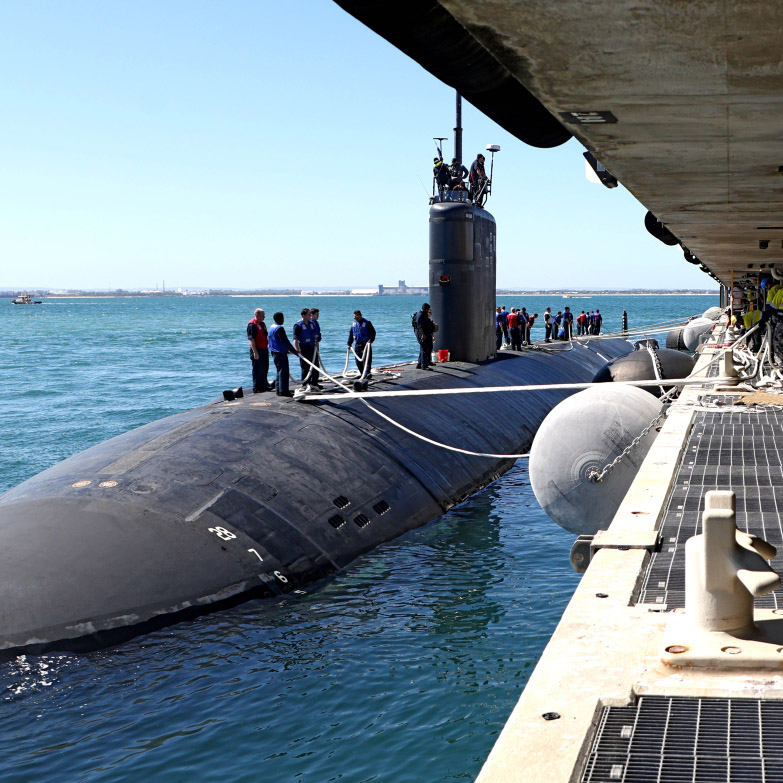
\includegraphics[width=6cm,height=6cm]{imgs/srf-w.jpg}} \\
    {\entrytableprojecthighlight%
	{SEA1180-1 NCIS-5 HMAS Coonawarra}
	{2023 to Present}
	{}
	{Maritime Design Lead for KBR}
	{Darwin, Northern Territory}
	{Client: Australian Department of Defence}
	{\vspace{1em}\begin{itemize}
		 \item Upgrade of existing wharf (including frontal pontoons) for homeporting of a number of new Arafura Class Offshore Patrol Vessels (ACOPVs).
		 \item Design solution required large frontal pontoons (to address Darwin's large tidal range) which were physically modelled to confirm behaviour in design events.
		 \item Technical oversight of maritime related construction support queries, including responding to RFIs, reviewing submittals and ensuring the Contractor met design intent.
		 \item Construction requires significant multi-disciplinary coordination due to the large amount of services required on the wharf.
		 \item Required to consider KBR's technical and commercial position when resolving issues arising on site.
	 \end{itemize}}
	} & \fcolorbox{black}{black}{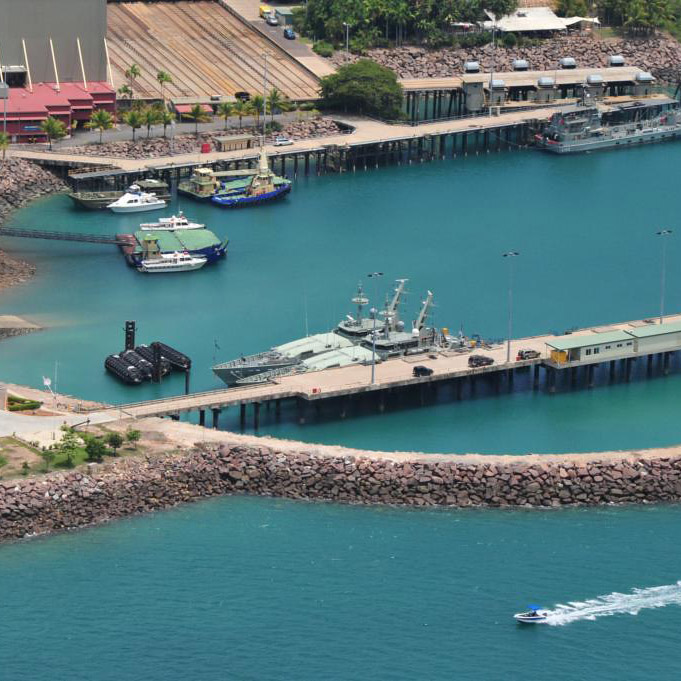
\includegraphics[width=6cm,height=6cm]{imgs/coonawarra.jpg}} \\
	{\entrytableprojecthighlight%
	{Australian Beach Erosion \& Coastal Flooding EWS}
	{2021 to 2023}
	{}
	{Research Associate for UNSW WRL}
	{Sydney, New South Wales}
	{}
	{\begin{itemize}
		\item Developed Early Warning System (EWS) for coastal storm hazards, publicly available \href{https://coastalews.wrl.unsw.edu.au/}{online} to deliver forecasts.
		\item System forecasts coastal flooding and beach erosion hazards across thousands of kilometres of shoreline across New South Wales and Western Australia.
		\item Responsible for developing methodology, models, data processing pipelines, automated workflows, and online dashboard.
		\item Gained an understanding of real-time forecasting systems over large areas, including scaling, monitoring and performance considerations.
		\item Liaised with and incorporated feedback from local, state and federal government project partners.
		\item Currently overseeing evaluation of system for to determine forecasting performance, with publication in preparation.
	 \end{itemize}}
	} & \fcolorbox{black}{black}{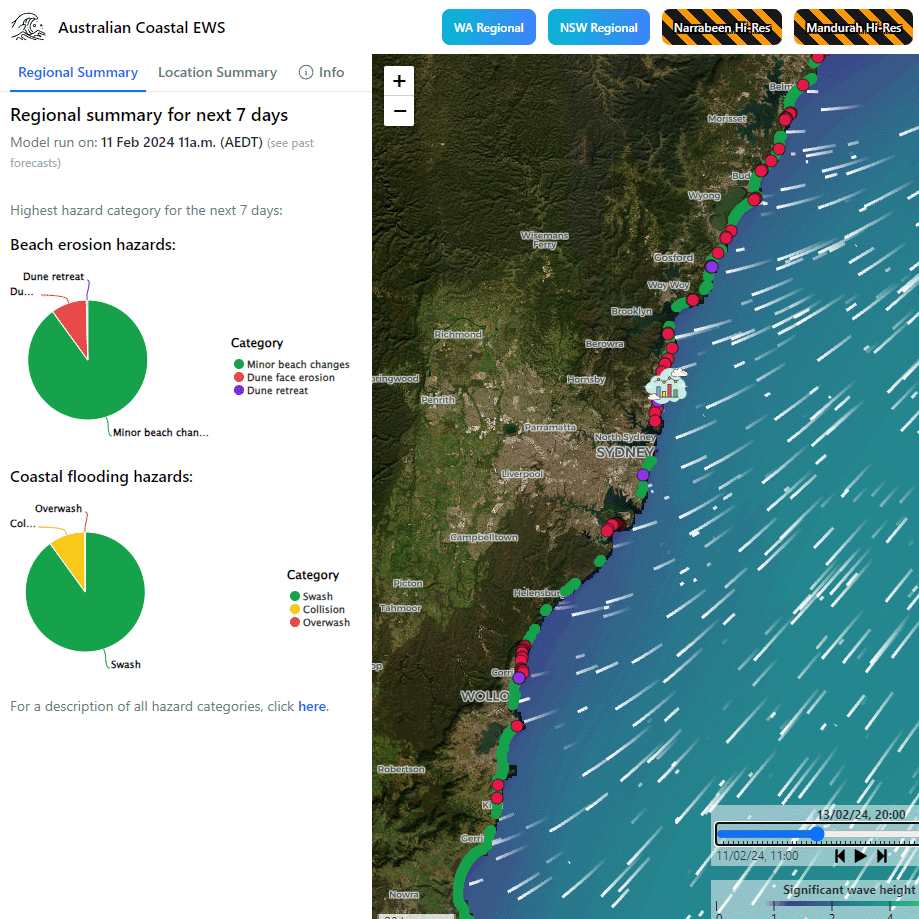
\includegraphics[width=6cm,height=6cm]{imgs/ews.png}} \\
	{\entrytableprojecthighlight%
	{Kingsford Smith Drive Upgrade}
	{2016 to 2018}
	{}
	{Maritime Structural Engineer for KBR}
	{Brisbane, Queensland}
	{Client: Lendlease and Brisbane City Council}
	{\vspace{1em}\begin{itemize}
		 \item Road widening along the Brisbane River, including a \SI{1.2}{\km} long marine retaining wall structure with cantilevered pedestrian and cycle path.
		 \item Responsibilities included performing detailed design calculations, writing design reports and specifications for the marine structure and associated works.
		 \item Design was required to consider a vessel impact design case, resulting in substantial loading onto the main structure and foundations.
		 \item Acquired substantial insitu and precast concrete detailing experience and was required to consider construction sequencing, creep, strut and tie design.
		 \item Designed a variety of smaller, miscellaneous structures, such as stone monument foundation, handrails, retaining walls, walkways and signs.  
		 \item Gained significant experience in a multi-disciplinary team, requiring coordination between roads, drainage, geotechnical, architectural, and electrical disciplines.
	 \end{itemize}}
	} & \fcolorbox{black}{black}{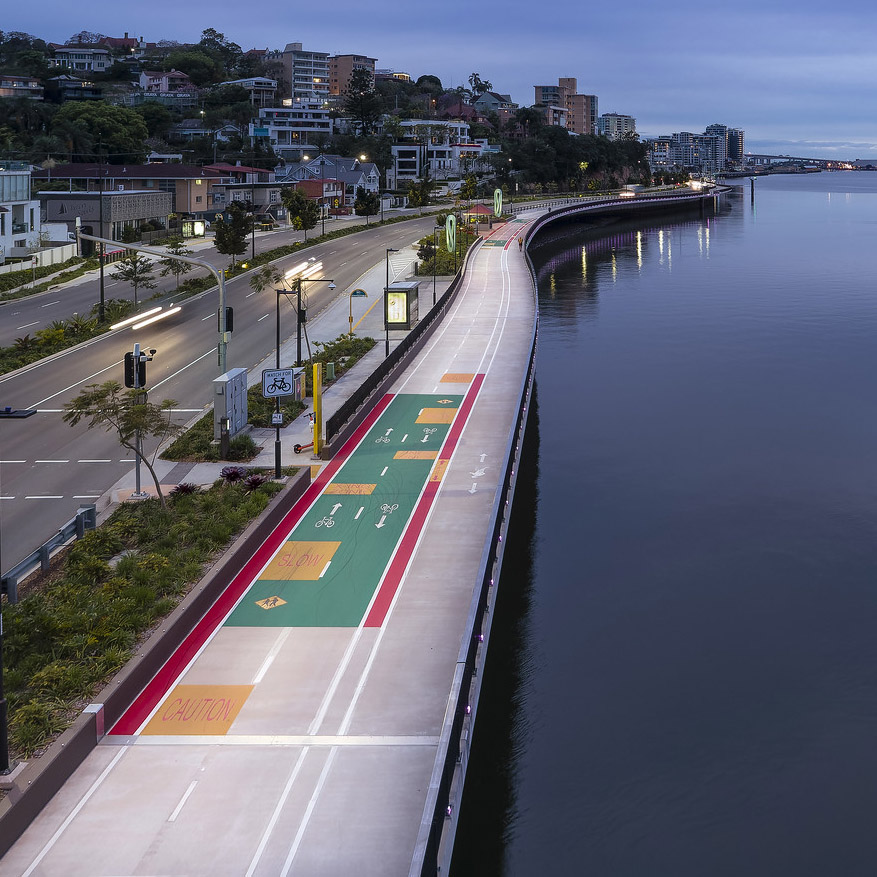
\includegraphics[width=6cm,height=6cm]{imgs/ksd.jpg}} \\
	% {\entrytableprojecthighlight%
	% {Townsville Port Inner Harbour Expansion (TPIX)}
	% {2012 to 2013}
	% {}
	% {Maritime Structural Engineer for KBR}
	% {Townsville, Queensland}
	% {Client: Port of Townsville}
	% {\begin{itemize}
	% 	 \item Reconstruction and extension of Berth 10 to accommodate military, cruise and commercial shipping, the construction of a new multi-purpose passenger terminal, and upgrade of Berth 8 to accommodate Panamax sized ships.
	% 	 \item Completing structural detailed design calculations for Berth 8 and Berth 10 works, developing design drawing and documentation.
	% 	 \item Performed on-site supervision of works on site. Required to consider KBR's technical and commerical position while resolving site issues.
	%  \end{itemize}}
	% } & \fcolorbox{black}{black}{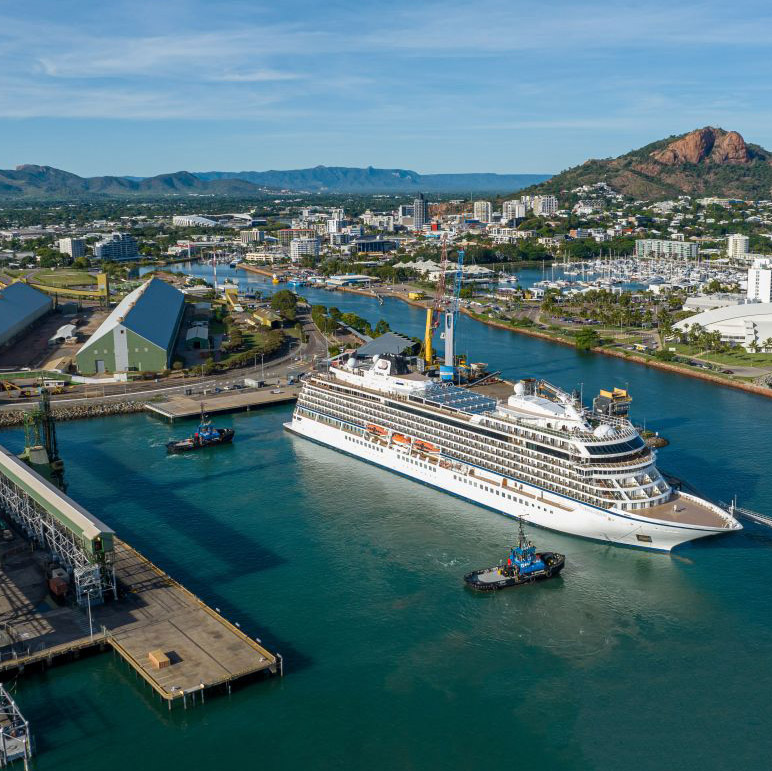
\includegraphics[width=6cm,height=6cm]{imgs/tpix.jpg}} \\
    \end{tblr}
\end{table}
\FloatBarrier

\section{Projects}

	% \entrytableproject%
	% {SEA1180-1 NCIS-5 HMAS Coonawarra}
	% {2022 to Present}
	% {}
	% {Maritime Design Lead for KBR (Client: Australian Department of Defence)}
	% {Cairns, Northern Territory}
	% {Upgrade of existing wharf (including frontal pontoons) for homeporting of new Arafura Class Offshore Patrol Vessels.}
	% {Technical oversight of maritime related construction support queries, and site inspections.}

	\entrytableproject%
	{Mackay Breakwater Maintenance Strategy Assessment}
	{2023 to Present}
	{}
	{Project Manager for KBR (Client: North Queensland Bulk Ports)}
	{Mackay, Queensland}
	{Assess NQBP's existing and alternative strategies to determine if there are more efficient maintanence approaches.}
	{Project budget, client communication, technical review and oversight of modelling reporting and deliverables.}

	\entrytableproject%
	{SEA3036-1PH4 Port Hera Infrastructure Project}
	{2023 to Present}
	{}
	{Maritime Design Lead for KBR (Client: Australian Department of Defence))}
	{Hera, Timor-Leste}
	{Concept and detailed design of wharf (\SI{100}{\m} long) and access bridge {\SI{140}{\m} long in seismic area.}}
	{Engineering design oversight of drawings and reports.}

	\entrytableproject%
	{Queens Beach South Coastal Protection Upgrade}
	{2022 to 2023}
	{}
	{Principal Coastal Engineer while at Moreton Bay Regional Council}
	{Brisbane, Queensland}
	{Upgrade of beach compartment with rock revetment (\SI{230}{\m} long), rock groynes and beach nourishment (\SI{13000}{\m\cubed}).}
	{Detailed design procurement, technical review and oversight of detailed design deliverables and specifications.}
	
	\entrytableproject%
	{TE Bonney Reserve \& Oyster Point Esp. Coastal Protection Upgrade}
	{2022 to 2023}
	{}
	{Principal Coastal Engineer at Moreton Bay Regional Council}
	{Beachmere \& Scarborough, Queensland}
	{Replacement of aging and informal seawalls at two locations (total length of \SI{435}{\m}) with new rock revetement.}
	{Detailed design procurement, technical review and oversight of detailed design deliverables and specifications.}

	\entrytableproject%
	{Woody Point Crockatt Park Seawall Renewal}
	{2022 to 2023}
	{}
	{Principal Coastal Engineer at Moreton Bay Regional Council}
	{Redcliffe, Queensland}
	{Replacement of an aging reinforced concrete vertical seawall (\SI{450}{\m} long) with new pre-cast concrete stepped seawall on a popular foreshore.}
	{Technical review and oversight of detailed design and specifications.}

	\entrytableproject%
	{Deception Bay Seawalls Condition Inspection \& Options Assessment}
	{2022 to 2023}
	{}
	{Principal Coastal Engineer at Moreton Bay Regional Council}
	{Deception Bay, Queensland}
	{Review of existing conditions of \SI{2}{\km} of ageing seawall and planning of repair and renewal works.}
	{Technical review and oversight of inspection works, including geotechnical investigation and statutory approvals, and options assessment.}

	\entrytableproject%
	{Charlish Park Seawall Renewal}
	{2022 to 2023}
	{}
	{Principal Coastal Engineer at Moreton Bay Regional Council}
	{Redcliffe, Queensland}
	{Proposed demolition of an ageing reinforced concrete stepped seawall and replacement with a rock armour revetment and crest wall.}
	{Technical review and oversight of detailed design and specifications.}

	\entrytableproject%
	{Flinders Parade Cliff Protection}
	{2021 to 2023}
	{}
	{Principal Coastal Engineer at Moreton Bay Regional Council}
	{Scarborough, Queensland}
	{Proposed stabilisation of approximately \SI{150}{\m} of coastal cliffs using groyne extension works and beach nourishment.}
	{Completing detailed design and documentation, including design of groyne and nourishment works.}

	\entrytableproject%
	{Kingsford Smith Drive Upgrade}
	{2016 to 2018}
	{}
	{Structural Engineer for KBR (Client: Lendlease and Brisbane City Council)}
	{Brisbane, Queensland}
	{Road widening along the Brisbane River, including a \SI{1.2}{\km} long marine retaining wall structure with cantilevered pedestrian and cycle path.}
	{Performing detailed design calculations, writing design reports and specifications for the marine structure and associated works.}

	\entrytableproject%
	{Dawson River Flood Study}
	{2015 to 2016}
	{}
	{Civil Engineer for KBR (Client: Banana Shire Council)}
	{Banana, Queensland}
	{Stage Two flood study to understand flooding impacts and mitigate future flood risks fors located on the Dawson River, Dee River and tributaries.}
	{Developed TUFLOW models and simulated future flood scenarios to identify areas of risk.}

	\entrytableproject%
	{Callide Dam Operation Study}
	{2015 to 2016}
	{}
	{Civil Engineer for KBR (Client: QLD Department of Energy and Water Supply, \& SunWater)}
	{Biloela, Queensland}
	{Investigated the feasibility of operating Callide Dam as a flood mitigation dam after the Feb 2015 flood event.}
	{Developing dam operational models to compared operating the dam using different procedures.}

	\entrytableproject%
	{Osborne No. 1 Berth Upgrade}
	{2015}
	{}
	{Maritime Structural Engineer for KBR (Client: Flinders Port Holdings)}
	{Adelaide, South Australia}
	{Wharf strengthening concept design to enable berth to accommodate larger vessels.}
	{Performing structural engineering concept development including design drawings and options report.}

	\entrytableproject%
	{Port of Brisbane Operations \& Maintenance Studies}
	{2014 to 2018}
	{}
	{Maritime Structural Engineer for KBR (Client: Port of Brisbane)}
	{Brisbane, Queensland}
	{Conditions assessment of various existing wharf structural components to evaluate residual life and propose maintenance strategies.}
	{Performing condition inspections (visual inspections in addition to non-destructive testing), performing structural capacity calculations and writing design report.}

	\entrytableproject%
	{Burrum Heads Boat Ramp and Car Trailer Park}
	{2014 to 2015}
	{}
	{Maritime Structural Engineer for KBR (Client: QLD Department of Transport and Main Roads)}
	{Burrum Heads, Queensland}
	{New recreational boating facility, including three-lane boat ramp, floating walkway, groyne, shore protection and drainage works.}
	{Performing detailed design drawings and documentation.}

	\entrytableproject%
	{Patterson River and Queenscliff Dredging Review}
	{2014 to 2015}
	{}
	{Coastal Engineer for KBR (Client: Parks Victoria)}
	{Melbourne, Victoria}
	{Optimization of Parks Victoria's dredging program at river entrances to maintain safe boating access.}
	{Completed numerical wave and sediment transport modelling for Port Philip bay.}

	\entrytableproject%
	{Legacy Way Residential Property Condition Surveys}
	{2014}
	{}
	{Structural Engineer for KBR (Client: Transcity Joint Venture)}
	{Indooroopilly, Queensland}
	{Two bored tunnels, \SI{4.6}{\km} long, carrying two motorway grade lanes of traffic in each direction between Toowong and Kelvin Grove.}
	{Engaging with local residents and conducting dilapidation surveys to assess potential impacts of underground construction works.}

	\entrytableproject%
	{Jazan Refinery Sea Water Cooling System}
	{2012 to 2014}
	{}
	{Civil Engineer for KBR (Client: Saudi Aramco)}
	{Jazan Economic City, Saudi Arabia}
	{Green-field oil refinery with a design capacity of \num{400000} barrels per day, using a seawater cooling system with a design flow of \SI{450000}{\m\cubed\per\hour}.}
	{Hydraulic modelling to confirm performance of open-channel structures, including development of operational procedures.}

	\entrytableproject%
	{Townsville Port Inner Harbour Expansion (TPIX)}
	{2012 to 2013}
	{}
	{Maritime Structures Engineer for KBR (Client: Port of Townsville)}
	{Townsville, Queensland}
	{Reconstruction and extension of Berth 10 to accommodate military, cruise and commercial shipping, the construction of a new multi-purpose passenger terminal, and upgrade of Berth 8 to accommodate Panamax sized ships.}
	{Completing structural calculations for Berth 8 and Berth 10 works, developing design drawing and documentation, and performing site supervision of construction works.}

	\entrytableproject%
	{Gorgon LNG Construction Support}
	{2011 to 2014}
	{}
	{Maritime Structures Engineer for KBR (Client: Kellogg Joint Venture Gorgon)}
	{Barrow Island, Western Australia}
	{Australia's largest single resource project, delivering 15.6 million tonnes per annum of LNG to Western Australia.}
	{Supporting construction works, in particular a large, steel, mechanical barge ramp used. Completing structural calculations, developing design drawings and documentation.}

	\entrytableproject%
	{Margate Seawall}
	{2011 to 2014}
	{}
	{Maritime Structures Engineer for KBR (Client: Moreton Bay Regional Council)}
	{Redcliffe, Queensland}
	{Detailed design of a 150 m segment of cast insitu, reinforced concrete, stepped seawall that uses vinyl sheet piling to limit the effects of scour.}
	{Completing detailed design and documentation of precast stepped seawall.}


% \begin{entrylist}
% 	\entry%
% 	{2014--15}
% 	{Wave Buoy Data Recovery, Processing and Management}
% 	{Deagon, Queensland}
% 	{\whileatfor{KBR}{Coastal Impacts Unit (Queensland Government)} \\
% 		Produced and documented MATLAB and Python scripts to consolidate historical wave buoy data.}
% \end{entrylist}



% \begin{entrylist}
% \entry%
% {2011--12}
% {Browse LNG Port Operability Study}
% {James Price Point, Western Australia}
% {\emph{Woodside Energy} \\
% Identified critical sea states for using wave hindcast data for use in mooring analysis.}
% \end{entrylist}



% \begin{sidewaystable}
\section{Projects Full List}
	\vspace{2em}
	\centering
	\footnotesize

	\setlength{\tymin}{40pt} % not so narrow columns
	\setlength{\tabcolsep}{8pt}
	% https://tex.stackexchange.com/a/373378
	% use \RaggedRight instead of \raggedright
	% \let\raggedright\RaggedRight

	\begin{tabulary}{\textwidth}{LLLLL}
	\toprule
	\textbf{Name} &
	  \textbf{Year} &
	  \textbf{Role} &
	  \textbf{Client} &
	  \textbf{Location} \\
	\midrule
	   Queens Beach South Coastal Protection Upgrade   & 2022 -- 2023 & Principal Coastal Engineer & Moreton Bay Regional Council & Brisbane, Queensland \\ 
	   TE Bonney Reserve \& Oyster Point Esp. Coastal Protection Upgrade   & 2022 -- 2023 & Principal Coastal Engineer & Moreton Bay Regional Council & Brisbane, Queensland \\ 
	\bottomrule
	\end{tabulary}

\end{sidewaystable}


% \section{Select Publications}
\entryitemindent{
  	\textbf{Leaman, C.K.}., Harley, M.D., Splinter, K.D., Thran, M.C., Kinsela, M.A., Turner, I.L., 2021. A storm hazard matrix combining coastal flooding and beach erosion. Coastal Engineering 170, 104001.

  	Tucker, T.A., Carley, J.T., Couriel, E.D., Phillips, M.S., \textbf{Leaman, C.K.}, 2019. Seawalls and acceptable beach width for public amenity. Australasian Coasts and Ports 2019 Conference: Future directions from 40 [degrees] S and beyond, Hobart, 10-13 September 2019 755.

	\textbf{Leaman, C.K.}, Splinter, K.D., Harley, M.D., Turner, I.L., Kinsela, M.A., 2019. Could an early warning system have forecast the impacts of a recent coastal erosion event along the SE Australian coast? Australasian Coasts and Ports 2019 Conference: Future directions from 40 [degrees] S and beyond, Hobart, 10-13 September 2019 755.

	Stewart, J.P., \textbf{Leaman, C.K.}, 2013. Validation of dredge plume modelling inputs. Coasts and Ports 2013: 21st Australasian Coastal and Ocean Engineering Conference and the 14th Australasian Port and Harbour Conference 715.

	A full list of publications can be found on \href{https://scholar.google.com/citations?user=LCvsG40AAAAJ&hl=en}{Google Scholar.}
}


% remove any extra blank pages
% https://stackoverflow.com/a/62581982
% \let\clearpage\relax

% \newpage

\section{Volunteer}



\entrytable%
{Northern Chapter Comittee Member}
{Nov 2024 to Present}
{(\difftoday{2024}{11}{01})}
{PIANC Northern Chaper}
{Brisbane, Queensland}
{\begin{itemize}
\item PIANC is the leading partner for government and private sector in the development of ports, waterways and coastal areas
\item Responsible for organising professional development and social events in QLD and NT.
	\end{itemize}
}


\entrytable%
{QLD Comittee Member}
{Nov 2024 to Present}
{(\difftoday{2024}{11}{01})}
{FutureNet Consult Australia}
{Brisbane, Queensland}
{\begin{itemize}
\item FutureNet provides young professionals with opportunities to engage with their peers from design, advisory and engineering industries.
\item Responsible for organising profession development and social events in QLD.
	\end{itemize}
}

\entrytable%
{PhD Student Representative}
{Jan 2019 to Dec 2020}
{(2 years)}
{UNSW WRL Research Management Group (RMG)}
{Sydney, New South Wales}
{\begin{itemize}
\item The RMG identifies opportunities and addresses issues regarding WRL's research output.
\item Managing creation of WRL webpage to showcase current PhD students and provide information to prospective students.
\item Organising social events between research and project staff to encourage collaboration.
	\end{itemize}
}

\entrytable%
{Treasurer}
{Jan 2012 to Dec 2015}
{(3 years)}
{Young Engineers Australia Queensland}
{Brisbane, Queensland}
{\begin{itemize}
\item YEAQ is a special interest group of Engineers Australia aimed at supporting young engineers.
\item Budgeted, managed and monitored the group's finances
\item Attracted over \$25,000 in industry sponsorship during the '13--'14 financial year.
\item Advised the committee on strategy to ensure events and initiatives were financially feasible.
\item Responsible for financial administration; keeping up-to-date records and ensuring compliance with processes and procedures.
	\end{itemize}
}



% \begin{entrylist}
% \entry%
% {2012--15}
% {IMPACT (KBR Graduate Program)}
% {Brisbane, Australia}
% {\emph{Graduate Program Coordinator} \\
% IMPACT is a network of developing professionals with 0--7 years of experience within KBR.
% \begin{itemize}
% \item Involved on a state and national level to deliver training and social activities to graduates.
% \item Proposed and monitored budget for social activities.
% \item Coordinated Australia's participation in company-wide events, such as Green Week and Global Week.
% \end{itemize}}
% \end{entrylist}



% 
% \section{software}
% \begin{adjustwidth}{2cm}{}
% \vspace{-2\parskip}
% \begin{multicols}{4}
% DELFT3D\\
% MIKE21\\
% TUFLOW\\
% \\
% Python\\
% Excel VBA\\
% MATLAB\\
% \\
% AutoCAD\\
% \LaTeX\\
% ArcGIS\\
% \\
% Strand7\\
% Microstran\\
% STAAD Pro\\
% \end{multicols}
% \vspace{-3\parskip}
% \end{adjustwidth}

\end{document}
